\documentclass{beamer}
\usetheme{CambridgeUS}
\usecolortheme{dolphin}
\usepackage{tikz}
\usepackage{amsmath}
\usepackage{graphicx}
\usepackage{pgffor} % Para loops

\title{Introdução a Processos Estocásticos}
\subtitle{Exemplo: Processo de Poisson}
\author{Prof. Jair Donadelli}
\institute{UFABC}
\date{\today}

\begin{document}

%------------------------------------------------
\begin{frame}
  \titlepage
\end{frame}
%------------------------------------------------

\begin{frame}{Intuição: Chegada de Clientes}
Imagine um café: os clientes chegam em instantes aleatórios.
\pause
\begin{itemize}
  \item O número de chegadas até o tempo $t$ é uma variável aleatória $X(t)$.
  \pause
  \item Cada dia observamos uma trajetória diferente do processo.
\end{itemize}
\end{frame}
%------------------------------------------------

\begin{frame}{Trajetória do Processo de Poisson (Simulada)}
\begin{center}
% Loop para incluir cada quadro com \only
\foreach \i in {1,...,10}{
    \only<\i>{
        \includegraphics[width=0.8\linewidth]{frames/frame_\i.png}
    }
}  
\end{center}
\pause
\begin{itemize}
  \item<7-> O processo é contínuo no tempo, mas o espaço de estados é discreto.
  \item<8-> Cada chegada aumenta $X(t)$ em +1.
  \item<9-> Cada trajetória é uma realização do processo estocástico.
\end{itemize}
\end{frame}
%------------------------------------------------

\begin{frame}{Distribuição de $X(t)$}
\begin{itemize}
  \item Para um processo de Poisson com taxa $\lambda > 0$:
  \[
  X(t) \sim \text{Poisson}(\lambda t)
  \]
  \item A probabilidade de $k$ chegadas até o tempo $t$:
  \[
  \mathbb{P}[X(t) = k] = e^{-\lambda t} \frac{(\lambda t)^k}{k!}, \quad k = 0,1,2,\dots
  \]
\end{itemize}

\begin{center}
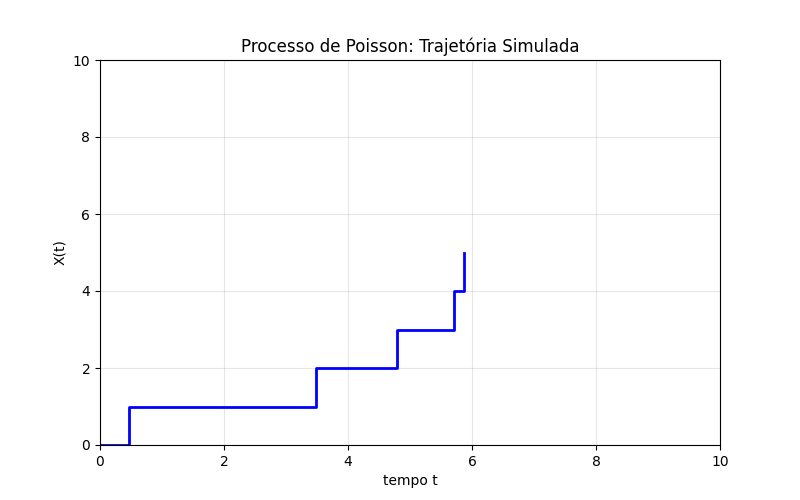
\includegraphics[width=0.6\linewidth]{frames/frame_6.png} % exemplo final da escada
\end{center}
\end{frame}
%------------------------------------------------

\begin{frame}{Conceitos-Chave do Processo de Poisson}
\begin{itemize}
  \item<1-> \textbf{Processo estocástico}: coleção $\{X(t), t \geq 0\}$.
  \item<2-> \textbf{Tempo contínuo, estados discretos}.
  \item<3-> \textbf{Trajetórias}: funções escada, não-decrescentes.
  \item<4-> \textbf{Propriedades}:
    \begin{itemize}
      \item<5-> Incrementos independentes.
      \item<6-> Incrementos estacionários.
    \end{itemize}
\end{itemize}
\end{frame}

\end{document}
